\begin{itemize}
 \item Forward / backward formulation
 \item Padding
\end{itemize}

\paragraph{Summary. }
\begin{itemize}
	\item Volume of size $W_i*H_i*D_i$ as input
	\item Requires four hyper-parameters :
    \begin{itemize}
    	\item number of filters (or kernels) K,
        \item spatial extent F,
        \item stride S,
        \item zero padding P
    \end{itemize}
	\item Produce a volume of size $W_o*H_o*D_o$ where :
    \begin{itemize}
		\item $W_o = \frac{W_i - F + 2*P}{S} + 1$
		\item $H_o = \frac{H_i - F + 2*P}{S} + 1$
		\item $D_o = K$
    \end{itemize}
    \item Number of weights equal to $F*F*D_i$ per filter
    \item Number of biases equal to 1 per filter
\end{itemize}


\paragraph{Padding. }

\begin{figure}
 \begin{center}
  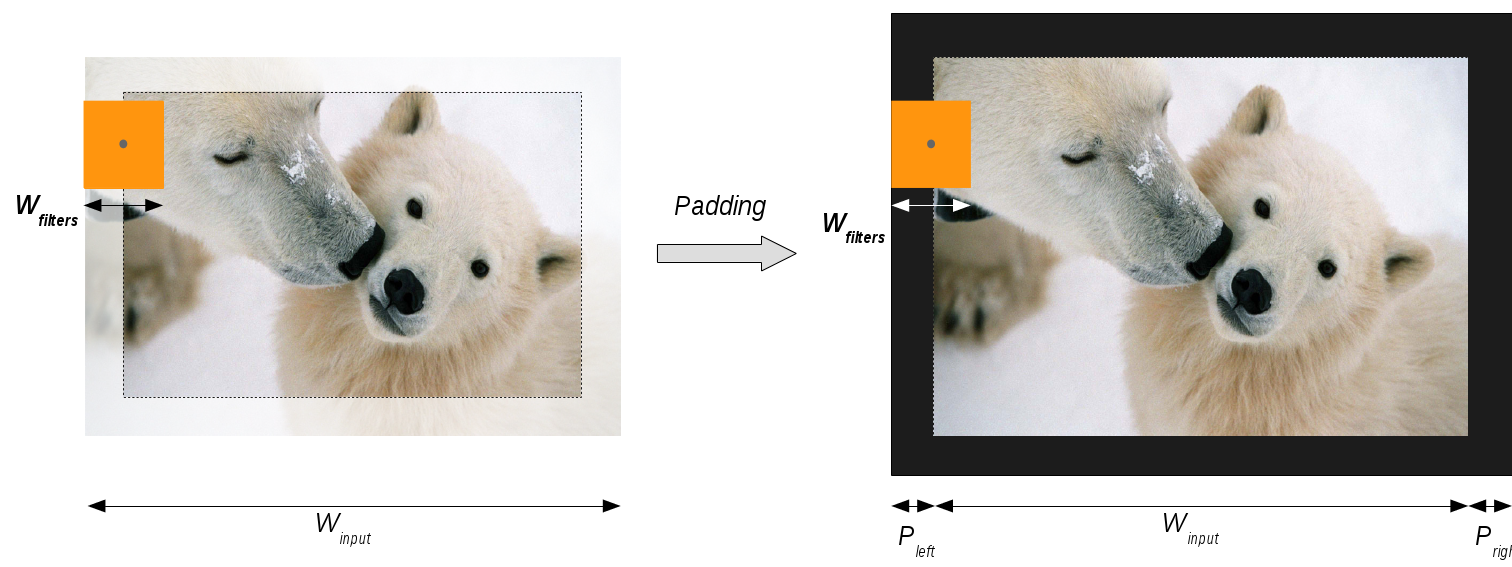
\includegraphics[width=16cm]{images/padding.png}
 \end{center}
  \caption{
  \label{fig:padding}
  Padding. Due to the filters width, the filters cannot be applied to the borders of the image. Padding consists in enlarging the 
  image by zeros, which enables the filters to be applied to the \textit{entire} image (including borders). 
  }
\end{figure}

In figure \ref{fig:padding}, we represent the padding (or ``zero-padding'') process. It consists in artificially augmenting the size of the input image (or map) in order to avoid border effects. Indeed, due to the width of the convolutional filters applied to the input maps, the center of the filters (represented as the grey dot in figure \ref{fig:padding}) cannot be at the border of the image. 
Convolutional padding is usually used to avoid a spatial reduction (downsampling) which is left for the pooling layers only. For instance, we have an image of size $30*30*3$ that we convolve using 128 filters of size $3*3*3$  with padding 0 and stride 1. The size of the output map will be $28*28*128$. If we had used a padding 1, it would have been $30*30*128$.

The total number of possible positions for the center of the filters is: 
\begin{align}
 W_{input} - W_{filters} + 1 \nonumber
\end{align}

However, if zeros are added at the border of the image, the center of the filters can be positionned at the border of the input image, so that the filters do not suffer from border effects. 
The total number of positions for the center of the filters is then: 
\begin{align}
 \underbrace{W_{input} + P_{left} + P_{right}}_{\textit{zero-padded image}} - W_{filters} + 1 \nonumber
\end{align}

Obviously, this process is applied in the same fashion no matter if the input is a set of maps or an 
image.




\paragraph{Volume of an output map. }

\begin{figure}
 \begin{center}
  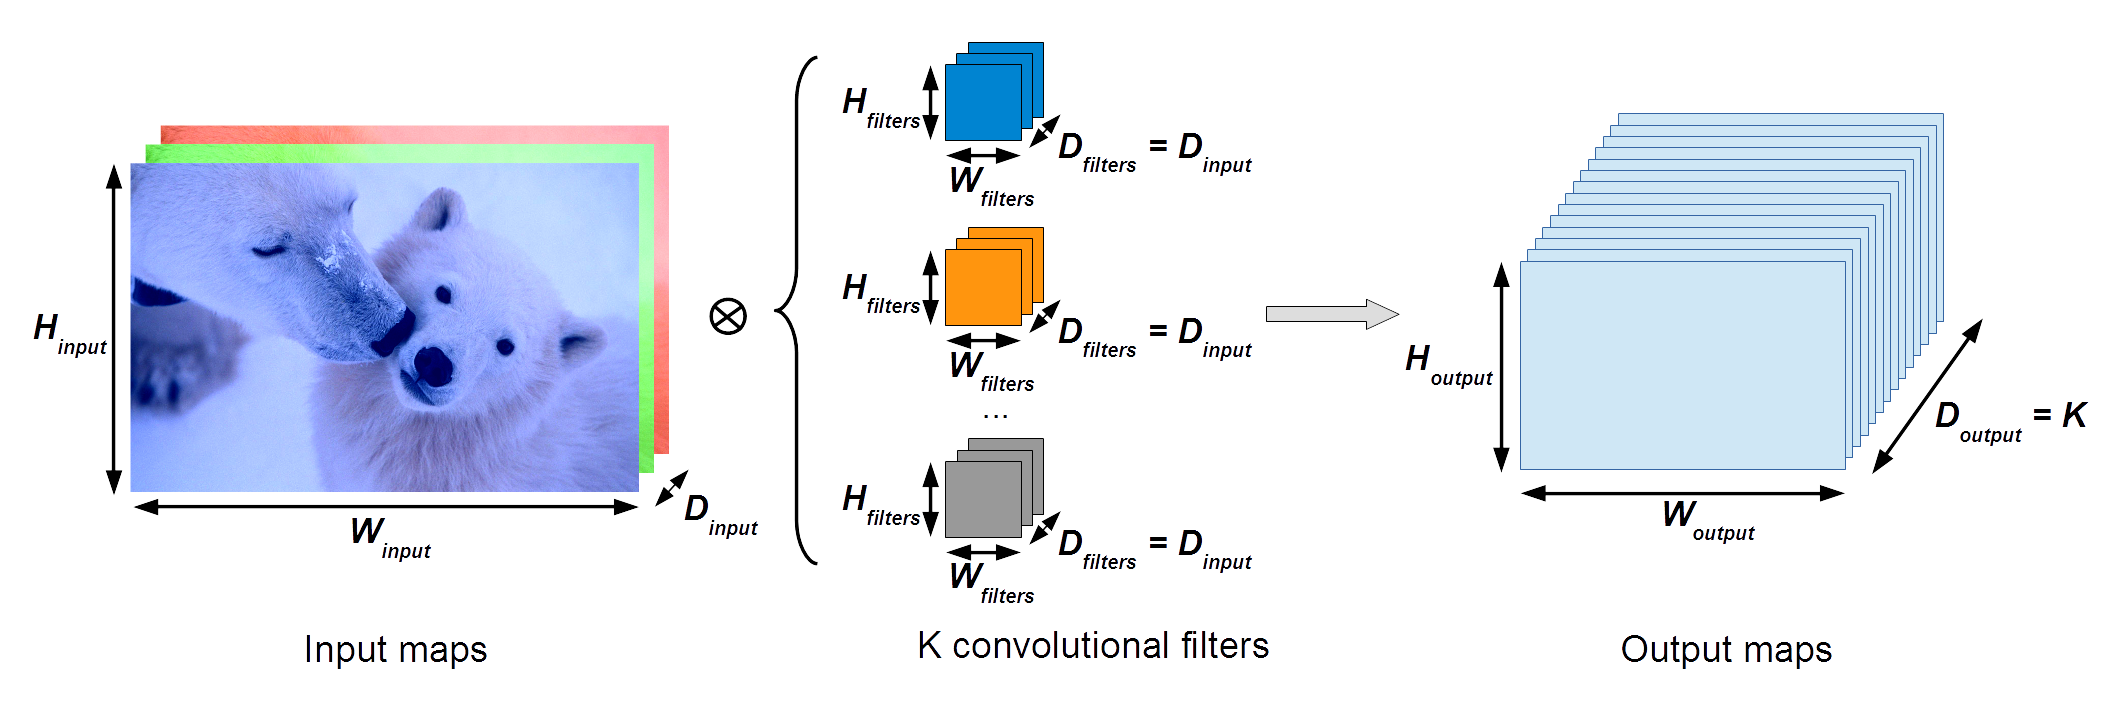
\includegraphics[width=16cm]{images/schema_conv.png}
 \end{center}
  \caption{
  \label{fig:conv}Convolution scheme. 
  }
\end{figure}

An output map is characterized by three parameters : depth, width and height. It is the result of a convolution apply to an input map made of the same parameters. For instance, an RGB image of size $227*227$ can be considered as an input map of size $[227*227*3]$.
In figure \ref{fig:conv}, we represent the general scheme for convolution. 
The width and height of the ouput map is used in particular when you want to compute the number of neurons which compose the fully connected layers. It is calculated as follow : 
\begin{align}
 W_{output} = \lfloor \frac{W_{input} + P_{left} + P_{right} - W_{filters}}{\delta_{filters}} \rfloor + 1 \nonumber
\end{align}
An equation can also be written for the height of the output map. However in the most popular cases width and height are equal.

For instance, the Alex net architecture that won the ImageNet challenge in 2012 take as input images of size $[227x227x3]$. The first convolutional layer uses neurons with receptive field size $W_{filters} = 11$, stride $\delta_{filters} = 4$ and padding $P_{left} = P_{right} = 0$. So the convolutional layer has an output volume of size $[55*55*96]$ ($\frac{227 + 0 + 0 - 11}{4} + 1 = 55$) and each of the $55*55*96$ neurons are connected to a region of size $[11*11*3]$.

The depth of the output map is however equivalent to the number of filters. Indeed, one map is produced for each of the $K$ filter banks; these response maps are then stocked as a 3D matrix.


\paragraph{Number of parameters. }

Using the real-world example from above, we can consider the first layer of AlexNet. The later is composed of 96 filters (or kernels) of size $[11*11*3]$, for a total of $96*11*11*3 = 34,848$ unique weights and 96 biases. In fact, each filter is applied to every group of $11*11*3$ pixels (considering stride and padding) to compute the final $55*55$ output map per filter, for a total of $55*55*96$ output. It is possible to find in the literature the concept of \textit{Parameter Sharing Scheme} to illustrate this fact.


\paragraph{Implementation. }

Also different implementations  of convolution can be found in the most famous libraries. For instance, the SpatialConvolutionMM from Torch nn constructs the Toeplitz matrix and does matrix multiplication. As the number of parameters does not change, one can try different implementations in order to improve efficiency.

\paragraph{Fully Connected layers. }

LeCun has once said that the concept of FC layers shouldn't be used when speaking about ConvNet, because FC layers can be seen as CONV layers with filters of size $[1*1]$.

\paragraph{Note. }

One can find some layers called TemporalConvolution, SpatialConvolution, or VolumetricConvolution. They are respectively used for processing acoustic signals (1D) or sequences of words, i.e. in Natural Language Processing, processing images (2 to 3D), or processing videos (4D).

\paragraph{Recent developments. }

\href{http://arxiv.org/abs/1412.6806}{Striving for Simplicity: The All Convolutional Net} proposes to discard the pooling layer in favor of architecture that only consists of repeated CONV layers. To reduce the size of the representation they suggest using larger stride in CONV layer once in a while.

